\documentclass[../machine_learning_scikit.tex]{subfiles}

\begin{document}

    \chapter{Training Simple Machine Learning Algorithms for Classification}

    So, we will see basic algorithms for classification and some other useful things.

    \section{Introduction}

    In this section we will make use of the first two algorithmically described machine learning algorithms for classification: the \textbf{perceptron} and \textbf{adaptive linear neurons}.

    Frist, we'll start by implementing a perceptron step by step in Python and training it to classify different flower species in the iris dataset.

    \begin{obs}
        Using this algorithm and discussing the basics of optimization using adaptive lienar neurons layse the groundwork for using more sophisticated classifiers.
    \end{obs}

    The goals of this chapter are the following:
    \begin{itemize}
        \item Building an understanding of machine learning algorithms
        \item Using pandas, NumPy, and Matplotlib to read in, process, and visualize data
        \item Implementing linear classifiers for 2-class problems in Python
    \end{itemize}

    \section{Artificial Neurons: Early Stages of Machine Learning}

    Warren McCulloch and Walter Pitts published the first concept of a simplified brain cell, the so-called McCulloch-Pitts (MCP) neuron, in 1943 (A Logical Calculus of the Ideas Immanent in Nervous Activity by W. S. McCulloch and W. Pitts, Bulletin of Mathematical Biophysics, 5(4): 115-133, 1943).

    \begin{obs}[\textbf{Biological Neurons}]
        Biological Neurons are interconnected nerve cells in the brain that are involved in the processing and transmiting of chemical and electrical signals.
    \end{obs}

    \begin{figure}[h]
        \begin{minipage}{\textwidth}
            \centering
            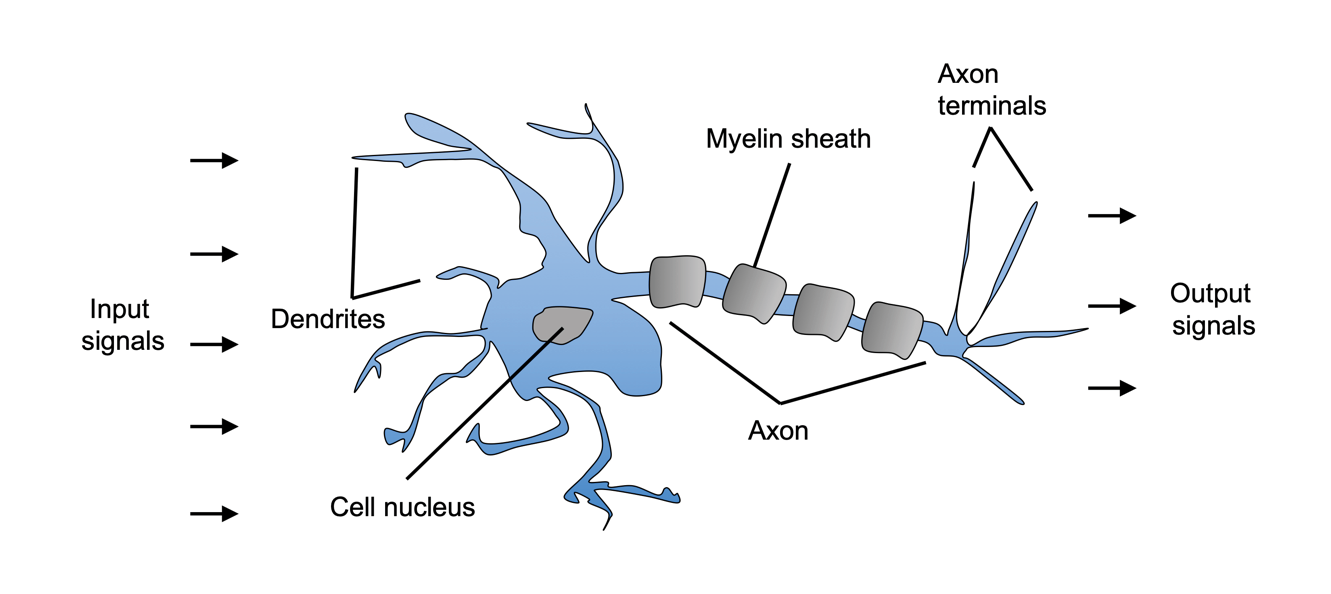
\includegraphics[scale=1]{images/nerve_cell.png} \\
            \caption{Biological Neuron.}
            \label{figure:biological_neuron}
        \end{minipage}
    \end{figure}

    \begin{idea}
        They described a nerve cell as a \textbf{simple logic gate with binary outputs}.
    \end{idea}

    Multiple signals arrive at the dendrites, they are then integrated into the cell body and, if the accumulated signals exceeds a certain threshold, an output signal is generated that will be passed on by the axon.

    \begin{obs}[\textbf{Perceptron Learning Rule}]
        Only a few years later, Frank Rosenblatt published the first concept of the \textbf{perceptron learning rule based} on the MCP neuron model (\textit{The Perceptron: A Perceiving and Recognizing Automaton} by F. Rosenblatt, Cornell Aeronautical Laboratory, 1957). With his perceptron rule, Rosenblatt \textit{proposed an algorithm that would automatically learn the optimal weight coefficients that would then be multiplied with the input features in order to make the decision of whether a neuron fires (transmits a signal) or not}.
    \end{obs}

    In the context of supervised learning and classification, \textit{such an algorithm could then be used to predict whether a new data point belongs to one class or the other}.

    \section{Formal Definition of an Artificial Neuron}

    We can put the idea of \textbf{articial neurons} into the context of a binary classification task with two classes: 0 and 1.

    \begin{mydef}[\textbf{Decision Function}]
        A \textbf{decision function} is a function $\cf{\sigma}{X}{\left\{0,1\right\}}$ that takes a linear combination of a certain input values (called $x$) and a corresponding weight vector (called $w$) , where $z$ is the net input:
        \begin{equation*}
            z=w_1x_1+w_2x_2+\dots+w_mx_m=\sum_{ i=1}^m w_ix_i
        \end{equation*}
        so, $\sigma(z)\in\left\{0,1\right\}$.
    \end{mydef}

    If the net input of a particular example is greater than a defined threshold (lets say $\vartheta\in\bbm{R}$, so $z\geq\vartheta$), we predict class 1, and class 0 otherwise. In the perceptron algorithm, the decision function, $\sigma(z)$ is a variant of a \textbf{unit step function}:
    \begin{equation*}
        \sigma(z)=\left\{
            \begin{array}{lr}
                1 & \textup{ if }z\geq\vartheta\\
                0 & \textup{ otherwise} \\
            \end{array}
        \right.
    \end{equation*}

    \begin{obs}
        We can modify the setup with a couple of steps. So, we make the \textbf{bias unit} $b=-\vartheta$, and we make:
        \begin{equation*}
            z'=w_1x_1+w_2x_2+\dots+w_mx_m+b=\vec{w}^T\vec{x}+b
        \end{equation*}
        And now replacing every input $z$ by $z'$ we obtain that:
        \begin{equation*}
            \sigma(z')=\left\{
                \begin{array}{lr}
                    1 & \textup{ if }z\geq0\\
                    0 & \textup{ otherwise} \\
                \end{array}
            \right.
        \end{equation*}
    \end{obs}

    \begin{obs}
        The transpose $A^T$ of matrix $A\in\mathcal{M}_{m\times n}$ is defined as:
        \begin{equation*}
            A^T=\left[
                \begin{array}{c c c c}
                    a_1^{(1)} & a_2^{(1)} & \cdots & a_n^{(1)} \\
                    a_1^{(2)} & a_2^{(2)} & \cdots & a_n^{(2)} \\
                    \vdots & \vdots & \ddots & \vdots \\
                    a_1^{(m)} & a_2^{(m)} & \cdots & a_n^{(m)} \\
                \end{array}
            \right]
        \end{equation*}
        where:
        \begin{equation*}
            A=\left[
                \begin{array}{c c c c}
                    a_1^{(1)} & a_2^{(1)} & \cdots & a_m^{(1)} \\
                    a_1^{(2)} & a_2^{(2)} & \cdots & a_m^{(2)} \\
                    \vdots & \vdots & \ddots & \vdots \\
                    a_1^{(n)} & a_2^{(n)} & \cdots & a_m^{(n)} \\
                \end{array}
            \right]
        \end{equation*}
    \end{obs}

    \begin{obs}[\textbf{Notation Problem}]
        This notation is horrible and differs from the one Mathmaticians use in all his textbooks, please, don't use this notation.
    \end{obs}

    \section{Perceptron Learning Rule}

    The whole idea behind the MCP neuron and Rosenblatt's thresholded perceptron model is to \textit{use a reductionist approach to mimic how a single neuron in the brain works}: \textbf{it either fires or it doesn't}. Thus, Rosenblatt's classic perceptron rule is fairly simple, and the perceptron algorithm can be summarized by the following steps:
    \begin{enumerate}
        \item Initialize the weights and bias unit to $0$ or small random numbers
        \item For each training example, $x^{(i)}$.
        \item Compute the output value, $\hat{y}^{(i)}$.
        \item Update the weight and bias unit.
    \end{enumerate}

    \begin{obs}[\textbf{Output Value}]
        Here, the \textbf{output value} is the \textbf{class label} \textit{predicted by the unit step function defined earlier}.
    \end{obs}

    The simultaneous update of each weight $w_j$ in the weight vector $\vec{w}$ can be formally written as:
    \begin{equation*}
        w_j\equiv w_j+\Delta w_j
    \end{equation*}
    and,
    \begin{equation*}
        b\equiv b+\Delta b
    \end{equation*}
    
    \begin{obs}[\textbf{Use of the Symbol $\equiv$}]
        Here, the symbol $\equiv$ states that the vlaue of the variable to the left is updated to that of the variable on the right.
    \end{obs}

    Where, the updated values (or \textbf{deltas}) are computed as follows:
    \begin{equation*}
        \Delta w_j=\eta(y^{(i)}-\hat{y}^{(i)})x_j^{(i)}
    \end{equation*}
    and,
    \begin{equation*}
        \Delta b=\eta(y^{(i)}-\hat{y}^{(i)})
    \end{equation*}

    \begin{obs}[\textbf{Notation Abuse}]
        This thing is absoultely ridicolus in terms of notation, the correct notation should be something like $\Delta w_j^{(i)}$, but since this variable is not going to be used anymore, we simply forgot about it, this is because in the process this variable is going to be updated every single time and we dont care about the different values depending on the $i$.
    \end{obs}

    Here, $\eta$ is a learning rate (usually between $0$ and $1$). $y^{(i)}$ is the \textbf{true class label} and $\hat{y}^{(i)}$ is the \textbf{predicted class label}.

    \begin{obs}
        The bias unit and all weights in the weight vector are updated simultaneously, which means that the predicted label $\hat{y}^{(i)}$ is not recomputed before the bias unit and all the wrights are updated via the respective update values, ,$\Delta w_j$ and $\Delta b$.
    \end{obs}

    \begin{exa}
        Concretely, for a two-dimensional dataset, we would write the update as:
        \begin{equation*}
            \begin{split}
                \Delta w_1&=\eta(y^{(i)}-\textup{output}^{(i)})x_1^{(i)}\\
                \Delta w_2&=\eta(y^{(i)}-\textup{output}^{(i)})x_2^{(i)}\\
                \Delta b&=\eta(y^{(i)}-\textup{output}^{(i)})\\
            \end{split}
        \end{equation*}
    \end{exa}

    \begin{enumerate}
        \item Before we implement the perceptron rule in Python, let's go through a simple thought experiment to illustrate how beautifully simple this learning rule really is. In the two scenarios where the perceptron predicts the class label correctly, the bias unit and weights remain unchanged, since the update values are 0:

        \item \textbf{When prediction is correct:}
        \begin{itemize}
            \item If $y^{(i)} = 0$ and $\hat{y}^{(i)} = 0$:
            \begin{align*}
            \Delta w_j &= \eta(0 - 0)x_j^{(i)} = 0 \\
            \Delta b &= \eta(0 - 0) = 0
            \end{align*}
            
            \item If $y^{(i)} = 1$ and $\hat{y}^{(i)} = 1$:
            \begin{align*}
            \Delta w_j &= \eta(1 - 1)x_j^{(i)} = 0 \\
            \Delta b &= \eta(1 - 1) = 0
            \end{align*}
        \end{itemize}

        \item \textbf{When prediction is wrong:}
        \begin{itemize}
            \item If $y^{(i)} = 0$ and $\hat{y}^{(i)} = 1$:
            \begin{align*}
            \Delta w_j &= \eta(0 - 1)x_j^{(i)} = -\eta x_j^{(i)} \\
            \Delta b &= \eta(0 - 1) = -\eta
            \end{align*}
            
            \item If $y^{(i)} = 1$ and $\hat{y}^{(i)} = 0$:
            \begin{align*}
            \Delta w_j &= \eta(1 - 0)x_j^{(i)} = \eta x_j^{(i)} \\
            \Delta b &= \eta(1 - 0) = \eta
            \end{align*}
        \end{itemize}

        \item To get a better understanding of the feature value as a multiplicative factor $x_j^{(i)}$, consider another example where $y^{(i)} = 1$, $\hat{y}^{(i)} = 0$, $\eta = 1$. Assume that $x_j^{(i)} = 1.5$ and this example is misclassified as class 0. In this case, we would increase the corresponding weight so that the net input $z = x_j^{(i)}w_j + b$ would be more positive the next time we encounter this example and thus more likely to be above the threshold of the unit step function to classify the example as class 1:
        \begin{align*}
        \Delta w_j &= (1 - 0) \times 1.5 = 1.5 \\
        \Delta b &= (1 - 0) = 1
        \end{align*}

        \item The weight update $\Delta w_j$ is proportional to the value of $x_j^{(i)}$. For instance, if we have another example $x_j^{(i)} = 2$ that is incorrectly classified as class 0, we will push the decision boundary by an even larger extent to classify this example correctly the next time:
        \begin{align*}
        \Delta w_j &= (1 - 0) \times 2 = 2 \\
        \Delta b &= (1 - 0) = 1
        \end{align*}

        \item The convergence of the perceptron is only guaranteed if the two classes are linearly separable, which means that the two classes can be perfectly separated by a linear decision boundary. If the two classes cannot be separated by a linear decision boundary, we can set a maximum number of passes over the training dataset (epochs) and/or a threshold for the number of tolerated misclassifications—the perceptron would never stop updating the weights otherwise.

        \item The perceptron receives the inputs of an example ($x$) and combines them with the bias unit ($b$) and weights ($w$) to compute the net input. The net input is then passed on to the threshold function, which generates a binary output of 0 or 1—the predicted class label of the example. During the learning phase, this output is used to calculate the error of the prediction and update the weights and bias unit.
    \end{enumerate}

    \section{Implementing a Perceptron Learning Algorithm in Python}

    Now, we will do an implementation of the Perceptron Rule in Python.

    \section{And Object-Oriented Perceptron API}

    We will take an object-oriented approach to defining the perceptron interface a a Python class, wich will allow us to initialize new Perceptron objects that can learn from data via a \lstinline|fit| method and make predictions via a separate \lstinline|predict| method.

    \begin{obs}
        We append an underscore \lstinline|_| to attributes that are not created upon the inicialization of the object, but we do this by calling the object's other methods, for example, \lstinline|self._w_|.
    \end{obs}

    The code is the following:

    \begin{lstlisting}[caption={Python Perceptron Rule Implementation.},label={code:perceptron_class_implementation}]
import numpy as np

class Perceptron:
    """Perceptron classifier.

    Parameters
    ------------
    eta : float
      Learning rate (between 0.0 and 1.0)
    n_iter : int
      Passes over the training dataset.
    random_state : int
      Random number generator seed for random weight
      initialization.

    Attributes
    -----------
    w_ : 1d-array
      Weights after fitting.
    b_ : Scalar
      Bias unit after fitting.
    errors_ : list
      Number of misclassifications (updates) in each epoch.

    """
    def __init__(self, eta=0.01, n_iter=50, random_state=1):
        self.eta = eta
        self.n_iter = n_iter
        self.random_state = random_state

    def fit(self, X, y):
        """Fit training data.

        Parameters
        ----------
        X : {array-like}, shape = [n_examples, n_features]
          Training vectors, where n_examples is the number of
          examples and n_features is the number of features.
        y : array-like, shape = [n_examples]
          Target values.

        Returns
        -------
        self : object

        """
        rgen = np.random.RandomState(self.random_state)
        self.w_ = rgen.normal(loc=0.0, scale=0.01, size=X.shape[1])
        self.b_ = np.float_(0.)
        self.errors_ = []

        for _ in range(self.n_iter):
            errors = 0
            for xi, target in zip(X, y):
                update = self.eta * (target - self.predict(xi))
                self.w_ += update * xi
                self.b_ += update
                errors += int(update != 0.0)
            self.errors_.append(errors)
        return self

    def net_input(self, X):
        """Calculate net input"""
        return np.dot(X, self.w_) + self.b_

    def predict(self, X):
        """Return class label after unit step"""
        return np.where(self.net_input(X) >= 0.0, 1, 0)
    \end{lstlisting}

    First, we will list the parameters and attributes of the code, in order to understand it better:
    \begin{itemize}
        \item \lstinline|eta|: Is a float, which represents the learning rate (a number between \lstinline|0.0| and \lstinline|1.0|).
        \item \lstinline|n_iter|: Is an integer, which is the number of passes over the training dataset.
        \item \lstinline|random_state|: It is an integer, which is a \textbf{random number generator seed} for random weight initialization.
    \end{itemize}

    \begin{mydef}[\textbf{Random Number Generator (RNG)}]
        A \textbf{random number generator (RNG) seed} is \textit{an initial value used by a computer algorithm to generate a sequence of pseudo-random numbers}. For random weight \textit{initialization in a neural network, this seed sets the starting point for the sequence of numbers used to initialize the model's weights and biases}.
    \end{mydef}

    The attributes are the following:
    \begin{itemize}
        \item \lstinline|w_|: It is a 1-dimensional array, which represents the weights after fitting.
        \item \lstinline|b_|: It is a float, which represents the bias unit after fitting.
        \item \lstinline|errors_|: It is a list, which is the number of misclassifications (or updates) in each \textbf{epoch}.
    \end{itemize}

    \begin{mydef}[\textbf{Epoch}]
        In machine learning, an \textbf{epoch} \textit{is one complete pass through the entire training dataset}. During a single epoch, \textit{the learning algorithm processes every training example once to update the model's internal parameters}. Training a model over multiple epochs \textit{allows it to progressively learn and refine its understanding of the data, with a well-tuned number of epochs balancing performance between underfitting and overfitting}.
    \end{mydef}

    In this code, we have three methods in the class Perceptron:
    \begin{itemize}
        \item \lstinline|__init__|: It initializes the parameters of the class, in this case, the \lstinline|eta| is setted to \lstinline|0.01|, \lstinline|n_iter=50| and \lstinline|random_state=1|.
        \item \lstinline|fit|: It is the code that fits the data in a dataset, given an array \lstinline|X| and another array \lstinline|y| of target values.
        \item \lstinline|net_input|: It calculates the net input of a dataset \lstinline|X|.
        \item \lstinline|predict|: It calculates the class label after a unit step of a dataset \lstinline|X|.
    \end{itemize}

    \begin{obs}[\textbf{Use of the Perceptron Implementation}]
        Using this perceptron implementation, we can initialize new Perceptron objects with a given learning rate, \lstinline|eta|, and the number of epochs, \lstinline|n_iter| (or iterations over the training dataset).
    \end{obs}

    Via the \lstinline|fit| method, we initialize the bias \lstinline|self.b_| to an initial value \lstinline|0| and the weights in \lstinline|self.w_| to a vector in $\bbm{R^m}$. Here, $m$ stands for the number of dimensions (features) in the dataset.

    \begin{obs}[\textbf{Decision of Initialization of Weight Vectors}]
        The \textbf{initial weight} vector contains small random numbers drawn from a normal distribution with a standard deviation of \lstinline|0.01| via \lstinline|rgen.normal(loc=0.0, scale=0.01, size=1 + X.shape[1])|, where \lstinline|rgen| is a NumPy random number generator seeded with a user-specified random seed so that results can be reproduced when desired.
    \end{obs}

    Technically, \textit{we could initialize the weights to zero (this is done in the original perceptron algorithm)}. However, if we did that, the \textbf{learning rate} $\eta$ (\lstinline|eta|) \textit{would have no effect on the decision boundary}. \textit{If all the weights are initialized to zero, the learning rate parameter affects only the scale of the weight vector, not the direction}. 

    \begin{obs}[\textbf{Use of Normal Distribution}]
        Our decision to draw the random numbers from a normal distribution—for example, instead of from a uniform distribution—and to use a standard deviation of \lstinline|0.01| was arbitrary; remember, we are just interested in small random values to avoid the properties of all-zero vectors, as discussed earlier.
    \end{obs}

    \begin{excer}
        As an optional exercise, you can change \lstinline|self.w_ = rgen.normal(loc=0.0, scale=0.01, size=X.shape[1])| to \lstinline|self.w_ = np.zeros(X.shape[1])| and \textit{run the perceptron training code presented in the next section with different values for \lstinline|eta|. You will observe that the decision boundary does not change}.
    \end{excer}

    After the weights have been initialized, the fit method loops over all individual examples in the training dataset and updates the weights according to the perceptron learning rule discussed in the previous section.

    \begin{obs}[\textbf{Prediction}]
        The \textbf{class labels are predicted by the predict method}, which is \textit{called in the fit method during training to get the class label for the weight update}; but \textit{predict can also be used to predict the class labels of new data after the model has been fitted}. Furthermore, we collect the number of misclassifications during each epoch in the \lstinline|self.errors_| list so that \textit{we can later analyze how well the perceptron performed during training}. The \lstinline|np.dot| function used in the \lstinline|net_input| method calculates the vector dot product, $wTx+bwTx+b$.
    \end{obs}

    \begin{idea}
        Instead of using \lstinline|NumPy| to calculate the vector dot product between two arrays, \lstinline|a| and \lstinline|b|, via \lstinline|a.dot(b)| or \lstinline|np.dot(a, b)|, we could also \textit{perform the calculation in pure Python} via \lstinline|sum([i * j for i, j in zip(a, b)])|. However, the advantage of using \lstinline|NumPy| over classic Python for loop structures is that \textbf{its arithmetic operations are vectorized}. \textit{Vectorization means that an elemental arithmetic operation is automatically applied to all elements in an array}. By formulating our arithmetic operations as a \textit{sequence of instructions on an array, rather than performing a set of operations for each element at a time, we can make better use of our modern central processing unit} (\textbf{CPU}) architectures with single instruction, multiple data (\textbf{SIMD}) support. Furthermore, \lstinline|NumPy| \textit{uses highly optimized linear algebra libraries, such as} \textbf{Basic Linear Algebra Subprograms} (\textbf{BLAS}) and \textbf{Linear Algebra Package} (\textbf{LAPACK}), that have been written in \lstinline|C| or \lstinline|Fortran|. Lastly, \lstinline|NumPy| also \textit{allows us to write our code in a more compact and intuitive way using the basics of linear algebra, such as vector and matrix dot products}.
    \end{idea}

    \section{Training of the Perceptron Algotithm on the Iris Dataset}

    \begin{obs}[\textbf{Restriction of Dimensions}]
        To \textit{test our perceptron implementation, we will restrict the following analyses and examples in the remainder of this section to two feature variables} (dimensions). Although the perceptron rule is not restricted to two dimensions, \textit{considering only two features—sepal length and petal length—allows us to visualize the decision regions of the trained model in a scatterplot}.
    \end{obs}

    \begin{idea}[\textbf{Restriction to Only Two Classes}]
        \textit{We will also only consider two flower classes, setosa and versicolor, from the Iris dataset for practical reasons} (remember, the \textbf{perceptron is a binary classifier}). However, the \textit{perceptron algorithm can be extended to multi-class classification using the one-versus-all (OvA) technique}.
    \end{idea}

    \subsection{OvA method for multi-class classification}

    We can extend any binary classifier to a multi-class problems using the method called \textbf{OvA} or \textbf{one-versus-rest} (\textbf{OvR}).

    \begin{mydef}[\textbf{One-versus-rest (OvR)}]
        The method \textbf{OvR} allows to extend any binary classifier to a multple classifier. To classify a new, unlabeled instance, we use our $n$ classifiers (where $n$ is the number of class labels) and \textit{assign the class label with the highest confidence to the instance}. For the perceptron, \textbf{we choose the class label associated with the largest absolute net input value}.
    \end{mydef}

    First, we use the \lstinline|pandas| library to load the Iris dataset directly from the \textbf{UCI Machine Learning Repository} into a \textbf{\lstinline|DataFrame| object} and \textit{print the last five lines via the tail method to confirm that the data loaded correctly}:

    \begin{lstlisting}[caption={Read Dataset from UCI.},label={code:reading_dataset}]
import os
import pandas as pd
s = 'https://archive.ics.uci.edu/ml/'\
    'machine-learning-databases/iris/iris.data'
print('From URL:', s)
#From URL: https://archive.ics.uci.edu/ml/machine-learning-databases/iris/iris.data
df = pd.read_csv(s,
                 header=None,
                 encoding='utf-8')
print(df.tail())
    \end{lstlisting}

    \begin{figure}[h]
        \begin{minipage}{\textwidth}
            \centering
            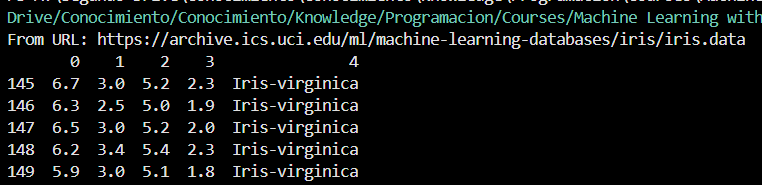
\includegraphics[scale=1]{images/tail_print_iris_dataset.png} \\
            \caption{Tail of the Iris Dataset.}
            \label{figure:tail_iris_dataset}
        \end{minipage}
    \end{figure}

    Next, \textit{we extract the first} \lstinline|100| \textit{class labels that correspond to the} \lstinline|50 Iris-setosa| and \lstinline|50 Iris-versicolor| \textit{flowers and convert the class labels into the two integer class labels} \lstinline|1| (\lstinline|versicolor|) and \lstinline|0| (\lstinline|setosa|), \textit{assigning them to a vector} \lstinline|y|. Similarly, \textit{we extract the first feature column} (\lstinline|sepal length|) \textit{and the third feature column} (\lstinline|petal length|) of those \lstinline|100| \textit{training examples and assign them to a feature matrix} \lstinline|X|, which we then \textit{visualize via a two-dimensional scatterplot}:

    \begin{lstlisting}[caption={Extraction and Visualization of Iris Dataset.},label=code:{extraction_and_visualization_iris_dataset}]
import matplotlib.pyplot as plt
import numpy as np
# select setosa and versicolor
y = df.iloc[0:100, 4].values
y = np.where(y == 'Iris-setosa', 0, 1)
# extract sepal length and petal length
X = df.iloc[0:100, [0, 2]].values
# plot data
plt.scatter(X[:50, 0], X[:50, 1],
            color='red', marker='o', label='Setosa')
plt.scatter(X[50:100, 0], X[50:100, 1],
            color='blue', marker='s', label='Versicolor')
plt.xlabel('Sepal length [cm]')
plt.ylabel('Petal length [cm]')
plt.legend(loc='upper left')
plt.show()
    \end{lstlisting}

    \begin{obs}[\textbf{Use of the Code}]
        Add this code to the remaining code.
    \end{obs}

    \begin{figure}[h]
        \begin{minipage}{\textwidth}
            \centering
            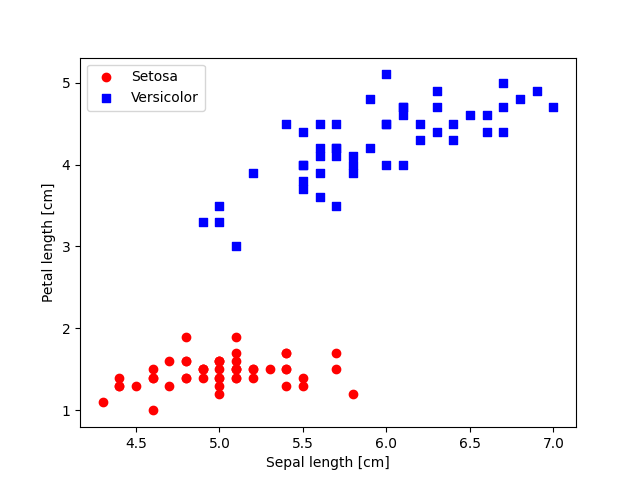
\includegraphics[scale=1]{images/iris_plot_seritosa_virginica.png} \\
            \caption{Plot of the Seritosa and Versicolor on the Iris Dataset.}
            \label{figure:iris_seritosa_versicolor_plot}
        \end{minipage}
    \end{figure}

    This plot shows the distribution of flower examples in the Iris dataset, along with the two feature axes: petal and sepal length.

    \begin{obs}
        In this subspace, a linear decision boundary should be sufficient to separate setosa from versicolor flowers.
    \end{obs}

    Thus, a linear classifier such as the perceptron should be able to classify the flowers in the Iris dataset perfectly.

    \subsection{Training the Algorithm}

    We will also plot the misclassification error for each epoch to check whether the algorithm converged and found a decision boundary that separates the two Iris flower classes:

    \begin{lstlisting}[caption={Training the Perceptron Algorithm with the Iris Dataset},label=code:training_perceptron]
import Perceptron
ppn = Perceptron(eta=0.1, n_iter=10)
ppn.fit(X, y)
plt.plot(range(1, len(ppn.errors_) + 1),
         ppn.errors_, marker='o')
plt.xlabel('Epochs')
plt.ylabel('Number of updates')
plt.show()
    \end{lstlisting}

    \begin{obs}
        In this scenario, since I put Perceptron in a different Python file, I have to import it in order to be able to use it.
    \end{obs}

    \begin{figure}[h]
        \begin{minipage}{\textwidth}
            \centering
            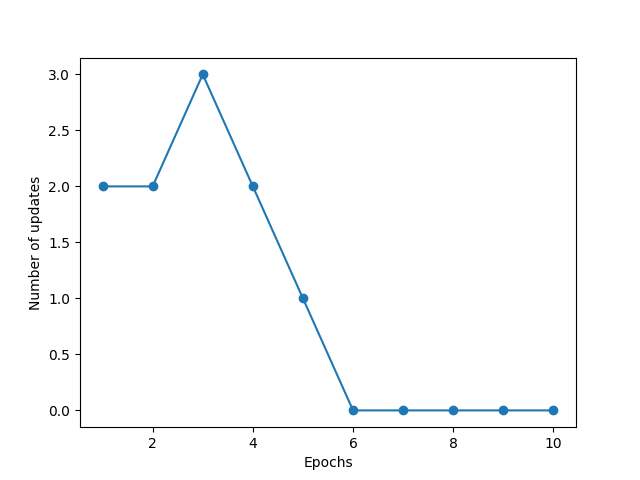
\includegraphics[scale=1]{images/epoch_plot_iris_dataset.png} \\
            \caption{Epoch Plot and Number of Updates on the Iris Dataset.}
            \label{figure:epoch_plot_iris_dataset}
        \end{minipage}
    \end{figure}

    \begin{obs}[\textbf{Convergence of the Perceptron}]
        As we can see, our \textbf{perceptron converged after the sixth epoch and should now be able to classify the training examples perfectly}.  
    \end{obs}

    Let's \textit{implement a small convenience function to visualize the decision boundaries for two-dimensional datasets}:

    \begin{lstlisting}[caption={Plotting Regions on the Iris Dataset},label=figure_plotting_regions]
from matplotlib.colors import ListedColormap

def plot_decision_regions(X, y, classifier, resolution=0.02):
    # setup marker generator and color map
    markers = ('o', 's', '^', 'v', '<')
    colors = ('red', 'blue', 'lightgreen', 'gray', 'cyan')
    cmap = ListedColormap(colors[:len(np.unique(y))])

    # plot the decision surface
    x1_min, x1_max = X[:, 0].min() - 1, X[:, 0].max() + 1
    x2_min, x2_max = X[:, 1].min() - 1, X[:, 1].max() + 1
    xx1, xx2 = np.meshgrid(np.arange(x1_min, x1_max, resolution),
                           np.arange(x2_min, x2_max, resolution))
    lab = classifier.predict(np.array([xx1.ravel(), xx2.ravel()]).T)
    lab = lab.reshape(xx1.shape)
    plt.contourf(xx1, xx2, lab, alpha=0.3, cmap=cmap)
    plt.xlim(xx1.min(), xx1.max())
    plt.ylim(xx2.min(), xx2.max())

    # plot class examples
    for idx, cl in enumerate(np.unique(y)):
        plt.scatter(x=X[y == cl, 0],
                    y=X[y == cl, 1],
                    alpha=0.8,
                    c=colors[idx],
                    marker=markers[idx],
                    label=f'Class {cl}',
                    edgecolor='black')
    \end{lstlisting}

    First, we \textit{define a number of \lstinline|colors| and \lstinline|markers| and create a colormap from the list of colors} via \lstinline|ListedColormap|. Then, we \textit{determine the minimum and maximum values for the two features and use those feature vectors to create a pair of grid arrays}, \lstinline|xx1| and \lstinline|xx2|, via \textit{NumPy's meshgrid function}. Since we trained our perceptron classifier on two feature dimensions, \textit{we flatten the grid arrays and create a matrix with the same number of columns as the Iris training subset so that we can use the predict method to predict the class labels lab of the corresponding grid points}.

    After \textit{reshaping the predicted class labels into a grid with the same dimensions as} \lstinline|xx1| and \lstinline|xx2|, we \textit{draw a contour plot via Matplotlib's contourf function, which maps the different decision regions to different colors for each predicted class in the grid array}:

    \begin{lstlisting}[caption={Plotting the Perceptron Info on the Iris Dataset},label=figure:plotting_perceptron_iris_dataset]
plot_decision_regions(X, y, classifier=ppn)
plt.xlabel('Sepal length [cm]')
plt.ylabel('Petal length [cm]')
plt.legend(loc='upper left')
plt.show()
    \end{lstlisting}

    \begin{figure}[h]
        \begin{minipage}{\textwidth}
            \centering
            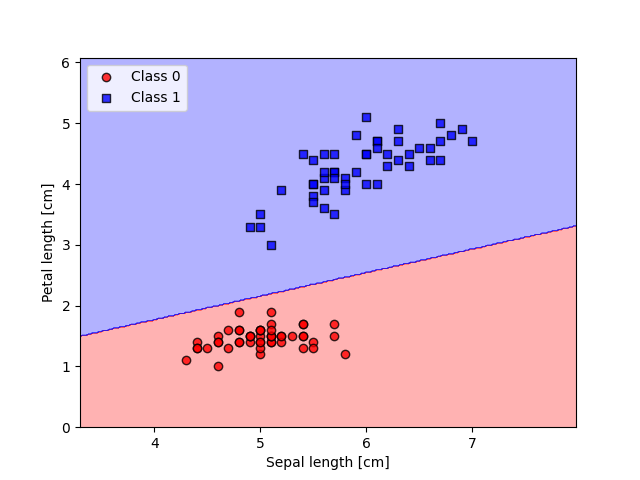
\includegraphics[scale=1]{images/perceptron_visual_implementation_iris_dataset.png} \\
            \caption{Perceptron Visual Classification on the Iris Dataset.}
            \label{figure:percepron_visual_classification_iris_dataset}
        \end{minipage}
    \end{figure}

    As we can see in the plot, the perceptron learned a decision boundary that can classify all flower examples in the Iris training subset perfectly.

    \begin{obs}[\textbf{Convergence of the Perceptron}]
        Although the \textit{perceptron classified the two Iris flower classes perfectly, convergence is one of its biggest challenges}. \textit{Rosenblatt proved mathematically that} the \textbf{perceptron learning rule converges if the two classes can be separated by a linear hyperplane}. However, \textit{if the classes cannot be separated perfectly by such a linear decision boundary, the weights will never stop updating unless we set a maximum number of epochs}. Interested readers can find a summary of the proof in the lecture notes at \href{https://sebastianraschka.com/pdf/lecture-notes/stat453ss21/L03_perceptron_slides.pdf}{Perceptron Slides}.
    \end{obs}

    \newpage

    \section{Adaptive Linear Neurons and the Convergence of Learning}

    \textbf{ADAptive LInear NEuron} (\textbf{Adaline}). \textbf{Adaline} was \textit{published by Bernard Widrow and his doctoral student Tedd Hoff only a few years after Rosenblatt's perceptron algorithm}, and it can be considered \textit{an improvement on the latter} (An Adaptive "Adaline" Neuron Using Chemical "Memistors", Technical Report Number 1553-2 by B. Widrow and colleagues, Stanford Electron Labs, Stanford, CA, October 1960).

    This algorithm is interesting because it ilustrates the key concepts of defining and minimizing a continuous loss function.

    \begin{obs}[\textbf{Use of Adaline}]
        This \textit{lays the groundwork for understanding other machine learning algorithms for classification}, such as logistic regression, support vector machines, and multilayer neural networks, as well as linear regression models.
    \end{obs}

    \begin{idea}[\textbf{Widrow-Hoff Rule}]
        The key difference between Adaline and the Perceptron is that weights are updated based on a linear activation function rather than a unit step function.

        This is called \textbf{Widrow-Hoff rule}.
    \end{idea}

    In Adaline, the linear activation function is the identity function of the net input, that is: $\sigma(z)=z$.

    \begin{obs}
        While the linear activation function is used for learning the weights, a threshold function is still applied to make the final prediction, which is similar to the unit step function covered earlier.
    \end{obs}

    \subsection{Main Differenes Between Perceptron and Adaline}

    \begin{figure}[h]
        \begin{minipage}{\textwidth}
            \centering
            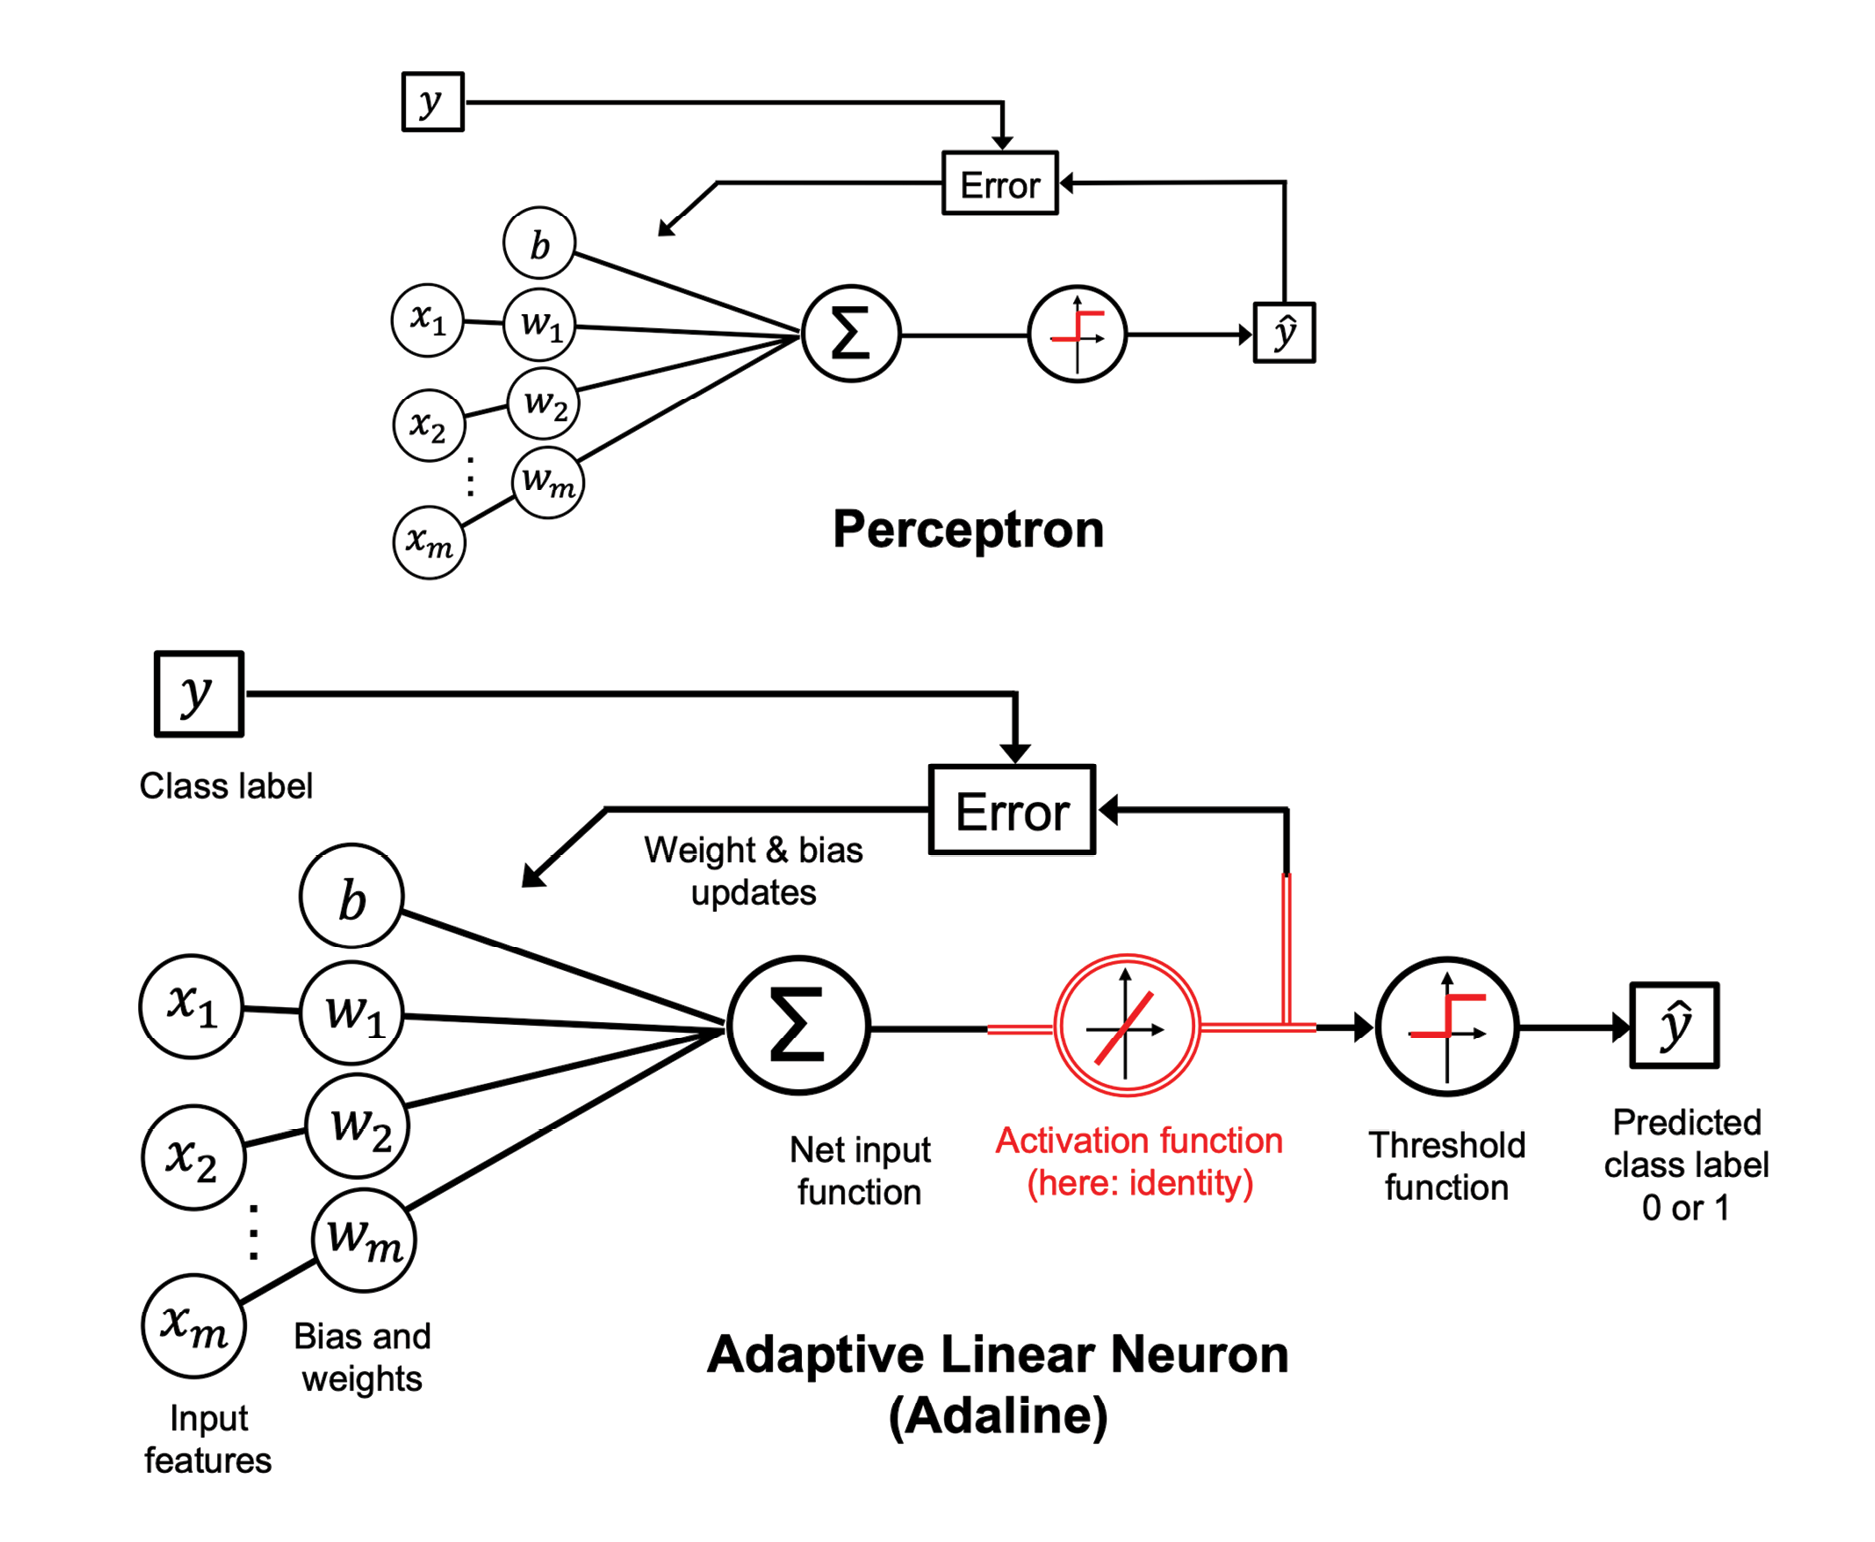
\includegraphics[scale=0.8]{images/perceptron_pipeline.png} \\
            \caption{Perceptron vs Adeline Work Flux.}
            \label{figure:perceptron_vs_adeline_work_flux}
        \end{minipage}
    \end{figure}

    \begin{obs}[\textbf{Perceptron vs Adeline}]
        The diagram shows that the \textit{Adaline algorithm compares the true class labels with the linear activation function's continuous-valued output to compute the model error and update the weights}, whereas the perceptron compares the true class labels to the predicted class labels.
    \end{obs}

    \subsection{Minimizing Loss Function with Gradient Descent}

    One of the key ingredients of supervised machine learning algorithms is a \textit{defined objective function that is optimized during learning}. This \textit{objective function is often a loss or cost function that we want to minimize}.

    \begin{obs}[\textbf{Loss Function in Adeline}]
        In the case of Adaline, the \textbf{loss function}, $L$, can be \textit{defined as the mean squared error (MSE) between the calculated outcome and the true class label}:
        \begin{equation*}
            L(w,b)=\frac{1}{n}\sum_{ i=1}^n\left(y^{(i)}-\sigma\left(z^{(i)}\right)\right)^2
        \end{equation*}
        It turns out that the continuous linear activation function makes the loss function differentiable. Also, this function is \textbf{convex}.
    \end{obs}

    \begin{mydef}[\textbf{Convex Function}]
        Let $X$ be a convex subset of a real vector space, and $\cf{f}{X}{\bbm{R}}$ a function. $f$ is called \textbf{convex} if for all $x_1,x_2\in X$ we have that:
        \begin{equation*}
            f\left(tx_1+(1-t)x_2 \right)\leq tf\left(x_1\right)+(1-t)f\left(x_2\right),\quad\forall t\in[0,1]
        \end{equation*}
    \end{mydef}

    The following image represents what a convex continuous function should look like:

    \begin{figure}[h]
        \begin{minipage}{\textwidth}
            \centering
            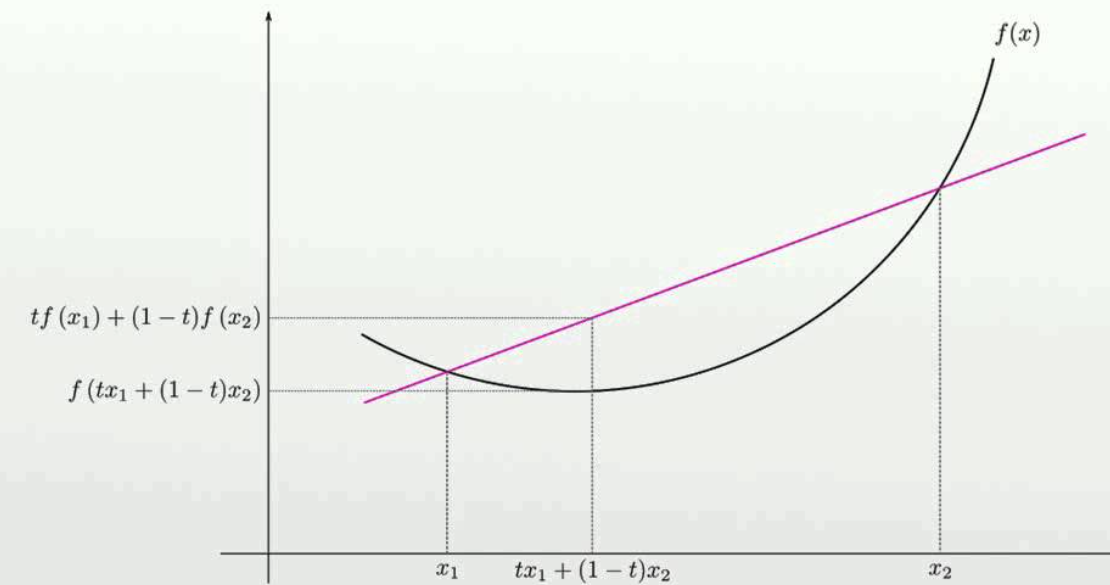
\includegraphics[scale=0.5]{images/convex_function_image.png} \\
            \caption{Convex Function.}
            \label{figure:convex_function}
        \end{minipage}
    \end{figure}

    \begin{obs}[\textbf{About Convex Functions}]
        When having a convex function and the inequality of the latter definition, the right side represents a straight line between $f(x_1)$ and $f(x_2)$. The argument of the function represents the line joining $x_1$ and $x_2$, so we compute its image under $f$.
    \end{obs}

    Due to the fact that the loss function is convex, we have a simple yet powerful optimization algorithm called \textbf{gradient descent} can be \textit{used to find the weights that minimize the loss function when classifying examples in the Iris dataset}.

    \begin{idea}[\textbf{Gradient Descent}]
        The idea behind \textbf{gradient descent} is to \textit{climb down a hill until a local or global loss minimum is reached}.
    \end{idea}

    \begin{figure}[h]
        \begin{minipage}{\textwidth}
            \centering
            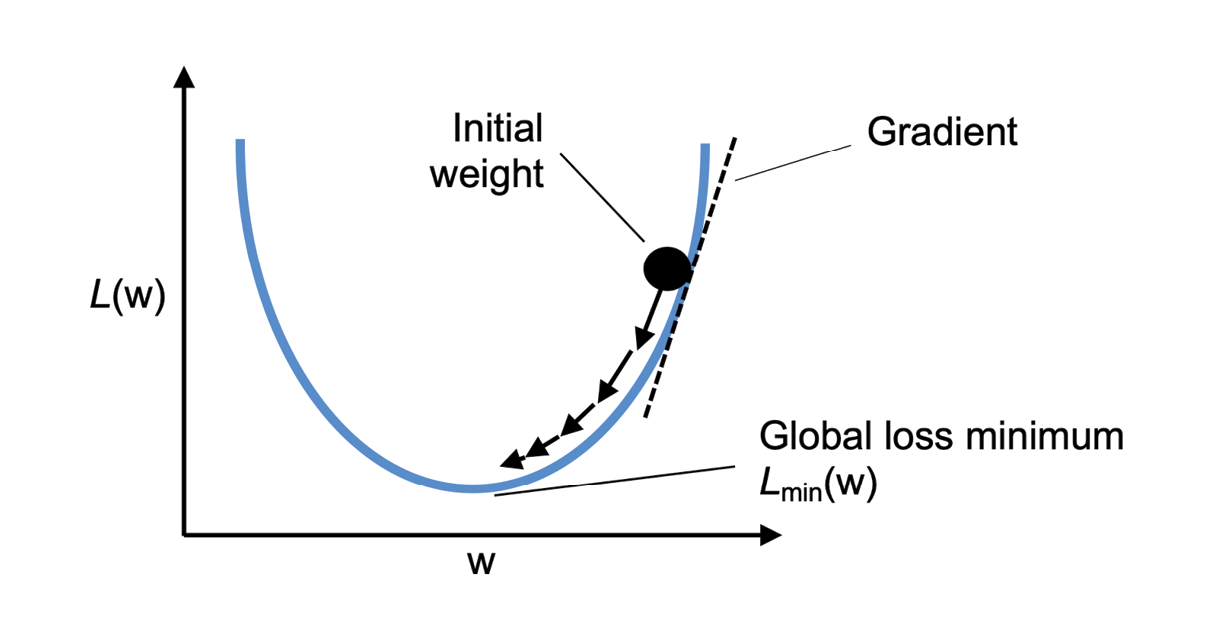
\includegraphics[scale=1]{images/gradient_descent.png} \\
            \caption{Gradient Descent.}
            \label{figure:gradient_descent}
        \end{minipage}
    \end{figure}

    The idea behind the algorithm is that on each iteration, a step is taken in the opposite direction of the gradient, where the step size is determined by the learning rate value and the slope of the gradient.

    \begin{obs}[\textbf{How Does Gradient Descent Works?}]
        \textbf{Gradient descent} \textit{updates each parameter by moving it in the direction that reduces the loss}:
        \begin{equation*}
            \vartheta-\nabla_{\vartheta}L(\vartheta)\rightarrow\vartheta
        \end{equation*}
        Here, $\vartheta$ represents any parameter of the model. But since we have two different parameters $w$ and $b$, we need to compute their individual gradients.
    \end{obs}

    Using gradient descent, the model parameters are updated by taking a step in the opposite direction of the gradient, $\nabla L(w,b)$ of the loss function $L(w,b)$:
    \begin{equation*}
        \begin{split}
            w&=w+\Delta w\\
            b&=b+\Delta b\\
        \end{split}
    \end{equation*}
    The parameter changes, $\Delta w$ and $\Delta b$ are defined as the negative gradient multiplied by the learning rate $\eta$:
    \begin{equation*}
        \begin{split}
            \Delta w &= -\eta\nabla_{w}L(w,b) \\
            \Delta b &= -\eta\nabla_{b}L(w,b) \\
        \end{split}
    \end{equation*}

    To compute the gradient of the loss function, compute the partial derivative of the loss function with respect to each weight, $w_j$:
    \begin{equation*}
        \frac{\partial L}{\partial w_j}=-\frac{2}{n}\sum_{ i=1}^n\left(y^{(i)}-\sigma(z^{(i)})\right)x_j^{(i)}
    \end{equation*}
    Similarly, compute the partial derivative of the loss with respect to the bias:
    \begin{equation*}
        \frac{\partial L}{\partial b}=-\frac{2}{n}\sum_{ i=1}^n\left(y^{(i)}-\sigma(z^{(i)})\right)
    \end{equation*}
    So, the weight updates becomes:
    \begin{equation*}
        \begin{split}
            \Delta w_j &= -\eta\frac{\partial L}{\partial w_j} \\
            \Delta b &= -\eta\frac{\partial L}{\partial b}\\
        \end{split}
    \end{equation*}

    \begin{obs}
        Let's recall that $\cf{L}{\bbm{R}^{n}\times\bbm{R}}{\bbm{R}}$, so its gradient with respect to $w$ and $b$ will be:
        \begin{equation*}
            \begin{split}
                \nabla_{w}L(w,b)&=\left[
                    \begin{array}{c}
                        \frac{\partial L}{\partial w_1}(w,b) \\
                        \frac{\partial L}{\partial w_2}(w,b) \\
                        \vdots \\
                        \frac{\partial L}{\partial w_j}(w,b) \\
                        \vdots \\
                        \frac{\partial L}{\partial w_n}(w,b) \\
                    \end{array}
                \right]\\
                \nabla_{b}L(w,b)&=\left[\frac{\partial L}{\partial b}(w,b) \right]=\frac{\partial L}{\partial b}(w,b)\\
            \end{split}
        \end{equation*}
        respectively. This makes perfect sense with the latter observation.
    \end{obs}

    \textbf{Note}: The MSE derivative involves calculus for weight adjustments.  

    \begin{obs}[\textbf{Batch Gradient Descent}]
        Although the Adaline learning rule looks identical to the perceptron rule, $\sigma(z^{(i)})$ where $z^{(i)}=w^Tx^{(i)}+b$ is a real number, not an integer class label.

        Furthermore, the \textit{weight update is calculated based on all examples in the training dataset (instead of updating the parameters incrementally after each training example), which is why this approach is often called} \textbf{batch gradient descent}. To be explicit and avoid confusion when discussing related concepts later in this section and throughout this course, this process is referred to as full \textbf{batch gradient descent}.
    \end{obs}

    \section{Implementing Adaline in Python}

    Since the perceptron rule and Adaline are very similar, we will take the perceptron implementation defined earlier and change the \lstinline|fit| method so that the \textit{weight and bias parameters are now updated by minimizing the loss function via gradient descent}:
    
    \begin{lstlisting}[caption={Adaline Implementation in Python.},label=code:adaline_implementation_python]
class AdalineGD:
    """ADAptive LInear NEuron classifier.

    Parameters
    ------------
    eta : float
        Learning rate (between 0.0 and 1.0)
    n_iter : int
        Passes over the training dataset.
    random_state : int
        Random number generator seed for random weight initialization.

    Attributes
    -----------
    w_ : 1d-array
        Weights after fitting.
    b_ : Scalar
        Bias unit after fitting.
    losses_ : list
      Mean squared error loss function values in each epoch.
    """
    def __init__(self, eta=0.01, n_iter=50, random_state=1):
        self.eta = eta
        self.n_iter = n_iter
        self.random_state = random_state

    def fit(self, X, y):
        """ Fit training data.

        Parameters
        ----------
        X : {array-like}, shape = [n_examples, n_features]
            Training vectors, where n_examples
            is the number of examples and
            n_features is the number of features.
        y : array-like, shape = [n_examples]
            Target values.

        Returns
        -------
        self : object

        """
        rgen = np.random.RandomState(self.random_state)
        self.w_ = rgen.normal(loc=0.0, scale=0.01,
                              size=X.shape[1])
        self.b_ = np.float_(0.)
        self.losses_ = []

        for i in range(self.n_iter):
            net_input = self.net_input(X)
            output = self.activation(net_input)
            errors = (y - output)
            self.w_ += self.eta * 2.0 * X.T.dot(errors) / X.shape[0]
            self.b_ += self.eta * 2.0 * errors.mean()
            loss = (errors**2).mean()
            self.losses_.append(loss)
        return self

    def net_input(self, X):
        """Calculate net input"""
        return np.dot(X, self.w_) + self.b_

    def activation(self, X):
        """Compute linear activation"""
        return X

    def predict(self, X):
        """Return class label after unit step"""
        return np.where(self.activation(self.net_input(X))
                        >= 0.5, 1, 0)
    \end{lstlisting}

    \begin{obs}[\textbf{Key Difference Between Adaline and Perceptron}]
        \textit{Instead of updating the weights after evaluating each individual training example, as in the perceptron}, \textbf{we calculate the gradient based on the whole training dataset}.
    \end{obs}

    For the bias unit, \textit{this is done via} \textbf{self.eta * 2.0 * errors.mean()}, where \textbf{errors is an array containing the partial derivative values} $\frac{\partial L}{\partial b}$ Similarly, we update the weights. However, note that the weight updates via the partial derivatives $\frac{\partial L}{\partial w_j}$ involve the feature values $x_j$, which we can compute by multiplying \lstinline|errors| with each feature value for each weight:  

    \begin{lstlisting}[caption={Computation of Partial Derivatives},label=code:computation_partial_derivatives]
for w_j in range(self.w_.shape[0]):
    self.w_[w_j] += self.eta * \
        (2.0 * (X[:, w_j]*errors)).mean()
    \end{lstlisting}

    To implement the weight update more efficiently without using a for loop, we can use a matrix-vector multiplication between the feature matrix and the error vector instead:  

    \begin{lstlisting}[caption={Weight Update Optimization.},label=code:weight_update_optimization]
self.w_ += self.eta * 2.0 * X.T.dot(errors) / X.shape[0]
    \end{lstlisting}

    \begin{obs}[\textbf{Activation Method}]
        The \lstinline|activation| method \textit{has no effect on the code since it is simply an identity function}. It \textit{is included to illustrate how information flows through a single-layer neural network: features from the input data, net input, activation, and output}.
    \end{obs}

    Later, we will learn about a logistic regression classifier that uses a \textit{non-identity, nonlinear activation function}.

    \begin{obs}[\textbf{Logistic Regression Model}]
        A \textbf{logistic regression model} \textit{is closely related to Adaline, with the only difference being its activation and loss function}.
    \end{obs}

    Similar to the previous perceptron implementation, we collect the loss values in a \lstinline|self.losses_ list| to \textit{check whether the algorithm converges after training}.

    \begin{obs}[Note]
        Matrix multiplication uses a vectorized approach for efficient computation.
    \end{obs}

    In practice, it often requires some experimentation to find a good learning rate, $\eta$, for optimal convergence. Let's choose two different learning rates, $\eta=0.1$ and $\eta=0.0001$, and plot the loss values versus the number of epochs to see how well the Adaline implementation learns from the training data.

    \subsection{Hyperparameters}

    The learning rate, $\eta$ (\lstinline|eta|), and the number of epochs (\lstinline|n_iter|) are hyperparameters of the perceptron and Adaline learning algorithms. Various techniques can help automatically find hyperparameter values that yield optimal classifier performance.

    Let's now plot the loss against the number of epochs for the two different learning rates:

    \begin{lstlisting}[caption={Loss for Two Different Learning Rates.},label=code:loss_two_different_learning_rates]
> fig, ax = plt.subplots(nrows=1, ncols=2, figsize=(10, 4))
...            np.log10(ada1.losses_), marker='o')
> ax[0].set_xlabel('Epochs'). ax[0].set_ylabel('log(Mean squared error)').
...            ada2.losses_, marker='o')
Set labels and title for the Adaline plot, then display it.
    \end{lstlisting}

    Using a \textit{learning rate that is too large can cause the mean squared error (MSE) to increase in every epoch because the updates overshoot the global minimum}. Conversely, \textit{a learning rate that is too small can lead to very slow convergence, requiring a large number of epochs to reach the minimum loss}.

    

\end{document}